% !TEX root = BLDC_Schrittmotoren_Technologie.tex
\renewcommand{\autoren}{Severin Schendel	}
\newpage

\subsection{Schrittmotoren}
\subsubsection{Allgemeines}
Schrittmotoren sind eine spezielle Bauform der Synchronmaschine, bei denen der Rotor als Permanentmagnet ausgeführt ist, während der Stator aus einem Spulenpaket besteht. Im Unterschied zum Synchronmotor hat der Schrittmotor eine große Zahl an Polpaaren. Die Drehung des Rotors kommt dadurch zustande, dass das elektromagnetische Feld der Stators Sprungweiße geschalten wird und sich um einen Schrittwinkel bewegt.

Zum Betrieb des Motors wird eine spezielle Ansteuereinheit(Treiber) benötigt.

\subsubsection{Arten des Schrittmotors}

Es gibt drei Grundtypen des Schrittmotors.

\begin{itemize}
	\item Reluktanzschrittmotor (VR)
	\item Permanenterregter Schrittmotor(PM)
	\item Hybridschittmotor(HY)
\end{itemize}

\begin{figure}[h]  % [h] bedeutet, dass das Bild genau an dieser Stelle im Text erscheint
\centering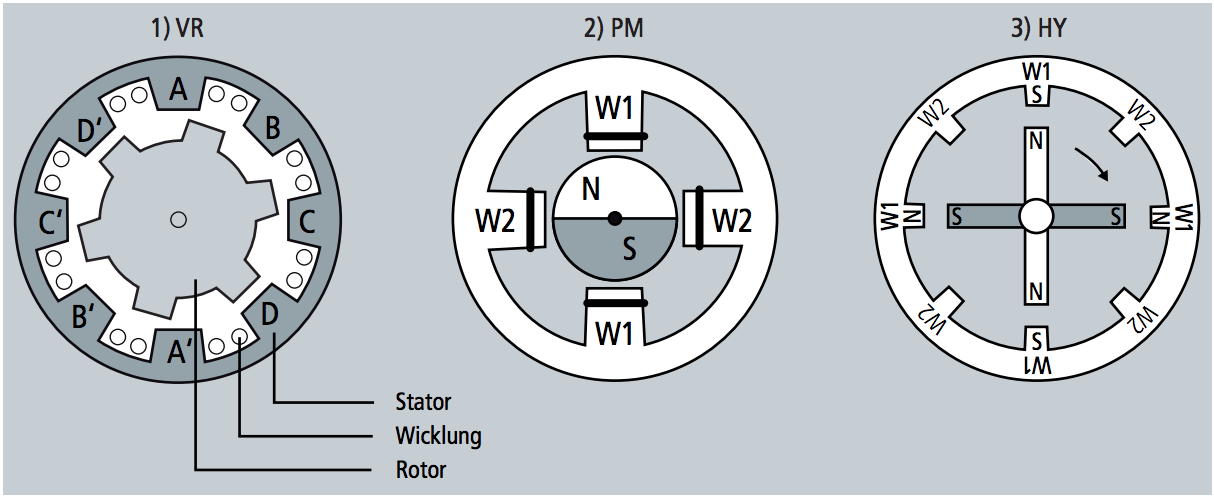
\includegraphics[width=1.0\textwidth]{images/Schrittmotortypen.png}
\caption{Schrittmotortypen \newline (Quelle: \cite{roboterKS_Bild})}
\label{robotKSys}
\end{figure}

Für unseren Anwendungsfall kommt nur der Hybridschrittmotor in Frage, aufgrund des Haltemomentes von 03 bis 1000 cNm und des kleinen Schrittwinkel von $0,36^\circ$.

\subsubsection*{Hybridschrittmotor}
Der Hybridschrittmotor vereint die positiven Eigenschaften des Reluktanzschrittmotor und des Permanenterregten Schrittmotor. Sein Rotor besteht aus einem axialen Permanentmagneten, an dessen Enden gezahnte Kappen befestigt sind. Beide sind um eine halbe Zahnbreite gegeneinander versetzt, so das sich Nord- und Südpole abwechseln.

\subsubsection{Arten der Ansteuerung}
Es gibt drei Möglichkeiten Schrittmotoren anzusteuern.
\begin{itemize}
	\item Vollschritt
	\item Halbschritt
	\item Mikroschritt
\end{itemize}

In unserem Fall wird der Mikroschrittbetrieb benötigt um ein genaues Positionieren zu ermöglichen.
\subsubsection*{Mikroschritt Betrieb}

\begin{quote}
	
Ein Schrittmotor führt Mikroschritte aus, wenn man die durch die Phasen fließenden Ströme nicht nur ein- oder ausschaltet, sondern in definierter Weise anwachsen und abnehmen läßt. Die Genauigkeit des Mikroschritts hängt davon ab, wieviele verschiedene Stromstärken vorgesehen sind und wie genau diese eingehalten werden. Die Theorie zeigt, daß eine sinusförmige Erregung am zweckmäßigsten ist. Es handelt sich dann eher um ein kontinuierliches Weiterdrehen als um ein ruckweises weiterschalten. Diese Betriebsweise hat einige Vorteile: 
\begin{itemize}
	\item ruhigerer Lauf
	\item keine Resonanzeffekte
	\item Geräuschminderung
	\item Schonung der Lager und ggf. nachgeordneter Antriebsteile
	\item bessere Auflösung bzw. Positioniergenauigkeit
\end{itemize}

Die sinuförmige Erregung erreicht man durch Stromsteuerung, genauer durch Beeinflussung der Referenzspannung. Für jede Wicklung wird eine Referenzspannung gebildet, deren Zeitverlauf aufeinanderfolgenden Sinushalbwellen  entspricht. Beide Referenzspannungen sind gegeneinander um 90° phasenverschoben.

\end{quote}




